\documentclass[12pt]{article}                         
\pagestyle{plain} %-- Document Set Up Command

%-- Document Setup & Layout
\usepackage{fancyhdr}
\usepackage{comment}
\usepackage{multicol}
\usepackage[
  letterpaper,
  left=0.8in,
  right=0.8in,
  textheight=9.5in,
  bmargin=0.75in  % Adjust this value to push the footer down
]{geometry}

%-- Color & Text Formatting
\usepackage[svgnames]{xcolor} 
\usepackage{textcomp}
\usepackage{ulem}
\usepackage{graphicx}

%-- Math Packages
\usepackage{amsmath}     
\usepackage{amsfonts}
\usepackage{amstext}
\usepackage{amssymb}
\usepackage{latexsym}
\usepackage{bm}

%-- Graphics and Figures
\usepackage{graphicx}    
\usepackage{tikz}
\usepackage{pgfplots}
\usepackage{circledtext}
\usepackage{float}
\usepackage{caption}
\usepackage{subcaption}
\usetikzlibrary{decorations.markings, arrows.meta}
%-- Tables
\usepackage{array}      
\usepackage{tabularx}

%-- Lists
\usepackage{enumitem}    
%\usepackage{enumerate}
\usepackage{tasks}

%-- TikZ Libraries
\usetikzlibrary{shapes.geometric} 
\pgfplotsset{compat=1.18}
\tikzset{
    phase arrow/.style={
        postaction={decorate,
            decoration={
                markings,
                mark=at position 0.1 with {\arrow{Stealth}},
                mark=at position 0.3 with {\arrow{Stealth}},
                mark=at position 0.7 with {\arrow{Stealth}},
                mark=at position 0.9 with {\arrow{Stealth}}
            }
        }
    },
    phase arrow left/.style={
        postaction={decorate,
            decoration={
                markings,
                mark=at position 0.1 with {\arrow{Stealth[reversed]}},
                mark=at position 0.3 with {\arrow{Stealth[reversed]}},
                mark=at position 0.7 with {\arrow{Stealth[reversed]}},
                mark=at position 0.9 with {\arrow{Stealth[reversed]}}
            }
        }
    }
}
%-- Header/Footer
\pagestyle{fancy}
\fancyhf{} % Clear all header and footer fields
\fancyhead[L]{Jack Lingbeck} % Left header with name
\fancyhead[R]{Janurary 30th, 2026} % Right header with date
\renewcommand{\headrulewidth}{0.4pt} % Horizontal line below the header
\rfoot{Page \thepage}
\lfoot{Homework 2 Unit 1}

\begin{document}
\large
\begin{center}
\fbox{\begin{tabular}{c}
\bf Math 675 Spring 2026: \\
\bf Homework 1 Unit ? \\
\bf Due Tuesday, Janurary 3rd, 2026\\
\end{tabular}}
\end{center}

\section*{Question 1:}
Consider the uncoupled system: $$x'=3x, y'=-y$$
\begin{enumerate}
    \item[a)] Solve the system explicitly for general initial conditions $(x(0),y(0))=(x_0,y_0)$.
    \begin{flalign*}
    \quad x'(t) &= 3x   & \quad y'(t) &= -y &\\
    \quad \frac{dx}{dt} &= 3x &  \quad \frac{dy}{dt} &= -y \\
    \quad \int \frac{1}{x} dx &= \int 3 dt & \quad \int \frac{1}{y} dy &= \int -1 dt \\
    \quad \ln|x| &= 3t + c_1 & \quad \ln|y| &= -t + c_2 \\
    \quad e^{\ln|x|} &= e^{3t + c_1} & \quad e^{\ln|y|} &= e^{-t + c_2} \\
    \quad x &= e^{3t} e^{c_1} & \quad y &= e^{-t} e^{c_2} \\
    \text{Solution: } x(t) &= c_1 e^{3t} & \text{Solution: } y(t) &= c_2 e^{-t} & \\
    \text{IC: } x(0) = x_0 & = c_1 & \text{IC: } y(0) = y_0 & = c_2 \\
    \text{Final Solution: } x(t) &= x_0 e^{3t} & \text{Final Solution: } y(t) &= y_0 e^{-t} & \\
\end{flalign*}
    \item[b)] Identify all equilibrium points of the system. \\
    $\left\{\begin{alignedat}{3} 3x  &&{}={} 0 \\ -y &&{}={} 0\end{alignedat}\right.
	\rightarrow
    \left\{\begin{alignedat}{3} x && = 0 \\ y && = 0\end{alignedat}\right.
	$ \\
    So like before, the only equilibrium point is at the origin $(0,0)$.
    \vspace{10cm}
    \item[c)] Using your explicit solution, determine the behavior of solutions as $t\to+\infty$:  
    Given out solutions from before: $x(t) = x_0 e^{3t}$ and $y(t) = y_0 e^{-t}$
    \begin{enumerate}
        \item[i)] initial conditions on the x-axis \\
        Using just $x=x_0 e^{3t}$, As $t\to +\infty$, \\
        If $x_0 > 0$ then $x(t) \to +\infty$ and if $x_0 < 0$ $x(t) \to -\infty$. \\\\
        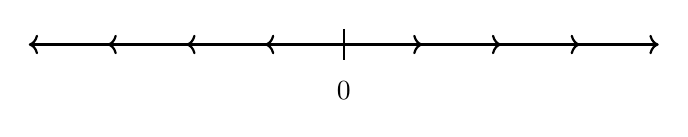
\begin{tikzpicture}
            \draw[thick, <->] (-4,0) -- (4,0);
            
            \draw[thick] (0,0.2) -- (0,-0.2) node[below=4pt] {0};
            
            \draw[thick, ->] (0.5,0) -- (1,0);
            \draw[thick, ->] (1,0) -- (2,0);
            \draw[thick, ->] (2,0) -- (3,0);
            
            \draw[thick, ->] (-0.5,0) -- (-1,0);
            \draw[thick, ->] (-1,0) -- (-2,0);
            \draw[thick, ->] (-2,0) -- (-3,0);
        \end{tikzpicture}

        \item[ii)] initial conditions on the y-axis \\
        Using just $y=y_0 e^{-t}$, As $t\to +\infty$, \\
        If $y_0 > 0$ then $y(t) \to 0$ and if $y_0 < 0$ $y(t) \to 0$. \\\\
        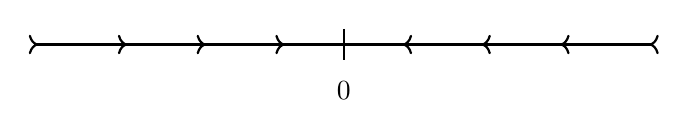
\begin{tikzpicture}
            \draw[thick, >-<] (-4,0) -- (4,0);
            
            \draw[thick] (0,0.2) -- (0,-0.2) node[below=4pt] {0};
            
            \draw[thick, <-] (0.75,0) -- (1,0);
            \draw[thick, <-] (1.75,0) -- (2,0);
            \draw[thick, <-] (2.75,0) -- (3,0);
            
            \draw[thick, <-] (-0.75,0) -- (-1,0);
            \draw[thick, <-] (-1.75,0) -- (-2,0);
            \draw[thick, <-] (-2.75,0) -- (-3,0);
        \end{tikzpicture}

        \item[iii)] initial conditions not lying on either axis \\
        \begin{minipage}{0.5\textwidth}
        
        \begin{itemize}
            \item If $t\to +\infty$ then solutions \\ approach the positive x-axis \\\\
            \item If $t\to -\infty$ then solutions \\ approach the negative x-axis
        \end{itemize}
        \end{minipage}
        \hfill
        \begin{minipage}{0.5\textwidth}
        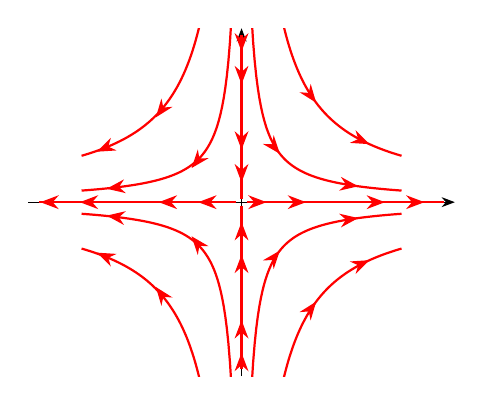
\begin{tikzpicture}
        \begin{axis}[
            width=7cm,
            height=6cm,
            axis lines = middle,
            samples=100,
            ymin=-5, ymax=5,
            xmin=-4, xmax=4,
            restrict y to domain=-10:10,
            xtick=\empty, ytick=\empty,
            axis line style={-Stealth}
        ]
            % Right Side (Pointing Right)
            \addplot[red, thick, phase arrow, domain=0.1:3] {1/x};
            \addplot[red, thick, phase arrow, domain=0.1:3] {4/x};
            \addplot[red, thick, phase arrow, domain=0.1:3] {-1/x};
            \addplot[red, thick, phase arrow, domain=0.1:3] {-4/x};

            % Left Side (Pointing Left)
            \addplot[red, thick, phase arrow left, domain=-3:-0.1] {1/x};
            \addplot[red, thick, phase arrow left, domain=-3:-0.1] {4/x};
            \addplot[red, thick, phase arrow left, domain=-3:-0.1] {-1/x};
            \addplot[red, thick, phase arrow left, domain=-3:-0.1] {-4/x};
            
            % Axis arrows
            \draw[red, thick, phase arrow ] (0.1, 0) -- (3.8, 0);     % Right
            \draw[red, thick, phase arrow left] (-3.8, 0) -- (-0.1, 0); % Left
            \draw[red, thick, phase arrow ] (0, 4.8) -- (0, 0.1);  % Down to origin
            \draw[red, thick, phase arrow ] (0, -4.8) -- (0, -0.1); % Up to origin
        \end{axis}
        \end{tikzpicture}
        \end{minipage} \\
    \item[d)] We can see from the behavior of the solutions as $t\to +\infty$ and $t\to -\infty$
    that the equilibrium point at the origin is a saddle point. This is because along the x-axis,
    the solutions diverge away from the origin, while along the y-axis, the solutions converge towards the origin. \\\\
    We can also see this as we take limits to positive and negitive \\ infinity of $x(t)=x_0 e^{3t}$ and $y(t)=y_0 e^{-t}$
    similar to what we have above, \\ As $t\to +\infty$, $x(t) \to +\infty$ and $y(t) \to 0$, \\ As $t\to -\infty$, $x(t) \to -\infty$ and $y(t) \to 0$. \\
    Because the limits for $y(t)$ are both $0$ yet the sign of infinity changes for $x(t)$, this tells us that this equilibrium point is a saddle point
    \vspace{5cm}
    \item[e)] Now we want to use Mathematica to plot the full phase portrait of this system. 
        \begin{figure}[H]
        \centering
        \includegraphics[width=0.4\textwidth]{Homework_2_Images/HW_2_Q1e.pdf}
        \end{figure}
        \end{enumerate}
\end{enumerate}

\section*{Question 2:}
Consider the uncoupled system: $$x'=3x, y'=-y$$
\begin{enumerate}
    \item[a)] 2
\end{enumerate}
\end{document}